\documentclass[12pt]{beamer}
\newenvironment{ConCodigo}[1]
  {\begin{frame}[fragile,environment=ConCodigo]{#1}}
  {\end{frame}}
\graphicspath{{Imagenes/}{../Imagenes/}}
\usepackage[utf8]{inputenc}
\usepackage[spanish]{babel}
\usepackage{hyperref}
\usepackage{etex}
\reserveinserts{28}
\usepackage{amsmath}
\usepackage{amsthm}
\usepackage{mathtools}
\usepackage{multicol}
\usepackage{multirow}
\usepackage{tabulary}
%\usepackage{tabularx}
\usepackage{booktabs}
\usepackage{nccmath}
\usepackage{biblatex}
\usepackage{epstopdf}
\usepackage{graphicx}
\usepackage{siunitx}
\sisetup{scientific-notation=true}
%\usepackage{fontspec}
\usepackage{lmodern}
\usepackage{float}
\usepackage[format=hang, font=footnotesize, labelformat=parens]{caption}
\usepackage[autostyle,spanish=mexican]{csquotes}
\usepackage{standalone}
\usepackage{tikz}
\usepackage[siunitx]{circuitikz}
\usetikzlibrary{arrows,patterns,shapes}
\usetikzlibrary{decorations.markings}
\usetikzlibrary{arrows}
\usepackage{color}
%\usepackage{beton}
%\usepackage{euler}
%\usepackage[T1]{fontenc}
\usepackage[sfdefault]{roboto}  %% Option 'sfdefault' only if the base font of the document is to be sans serif
\usepackage[T1]{fontenc}
\renewcommand*\familydefault{\sfdefault}
\DeclareGraphicsExtensions{.pdf,.png,.jpg}
\usepackage{hyperref}
\renewcommand {\arraystretch}{1.5}
\newcommand{\python}{\texttt{python}}
\usefonttheme[onlymath]{serif}
\setbeamertemplate{navigation symbols}{}
\usetikzlibrary{patterns}
\usetikzlibrary{decorations.markings}
\tikzstyle{every picture}+=[remember picture,baseline]
%\tikzstyle{every node}+=[inner sep=0pt,anchor=base,
%minimum width=2.2cm,align=center,text depth=.15ex,outer sep=1.5pt]
%\tikzstyle{every path}+=[thick, rounded corners]
\setbeamertemplate{caption}[numbered]
\newcommand{\ptm}{\fontfamily{ptm}\selectfont}
%Se usa la plantilla Warsaw modificada con spruce
\mode<presentation>
{
  \usetheme{Warsaw}
  \setbeamertemplate{headline}{}
  \useoutertheme{default}
  \usecolortheme{beaver}
  \setbeamercovered{invisible}
}
\AtBeginSection[]
{
\begin{frame}<beamer>{Contenido}
\normalfont\mdseries
\tableofcontents[currentsection]
\end{frame}
}

\usepackage{listings}
\lstset{ %
language=Python,                % choose the language of the code
basicstyle=\small,       % the size of the fonts that are used for the code
numbers=left,                   % where to put the line-numbers
numberstyle=\small,      % the size of the fonts that are used for the line-numbers
stepnumber=1,                   % the step between two line-numbers. If it is 1 each line will be numbered
numbersep=5pt,                  % how far the line-numbers are from the code
backgroundcolor=\color{white},  % choose the background color. You must add \usepackage{color}
showspaces=false,               % show spaces adding particular underscores
showstringspaces=false,         % underline spaces within strings
showtabs=false,                 % show tabs within strings adding particular underscores
frame=single,   		% adds a frame around the code
tabsize=2,  		% sets default tabsize to 2 spaces
captionpos=b,   		% sets the caption-position to bottom
breaklines=true,    	% sets automatic line breaking
breakatwhitespace=false,    % sets if automatic breaks should only happen at whitespace
escapeinside={\%},          % if you want to add a comment within your code
stringstyle =\color{magenta},
keywordstyle = \color{blue},
commentstyle = \color{green},
identifierstyle = \color{red}
}
\title{Tema 2 - Operaciones matemáticas básicas}
\subtitle{Técnicas de Interpolación III \\ Consideraciones sobre las técnicas de interpolación}
%\subsubtitle{Curso de Física Computacional}
\author[]{M. en C. Gustavo Contreras Mayén}
%\email{curso.fisica.comp@gmail.com}
%\ptsize{10}
\begin{document}
\maketitle
\fontsize{14}{14}\selectfont
\spanishdecimal{.}
\begin{frame}{Contenido}
\tableofcontents[pausesections]
\end{frame}
\section{Fenómeno de Runge}
\begin{frame}
\frametitle{Fenónemo de Runge}
Hasta el momento hemos revisado un par de estrategias para calcular un polinomio que pase por un conjunto de datos $(x_{i}, y_{i})$, pero hay que considerar un efecto importante al respecto: no siempre el mejor polinomio será aquel el de mayor grado $n$.
\\
\medskip
Veamos el siguiente ejemplo: sea la función:
\[ f(x) = \dfrac{1}{1 + 25 x^{2}}\]
\end{frame}
\begin{frame}
\frametitle{Gráfica de la función $f(x)$}
\begin{figure}
	\centering
	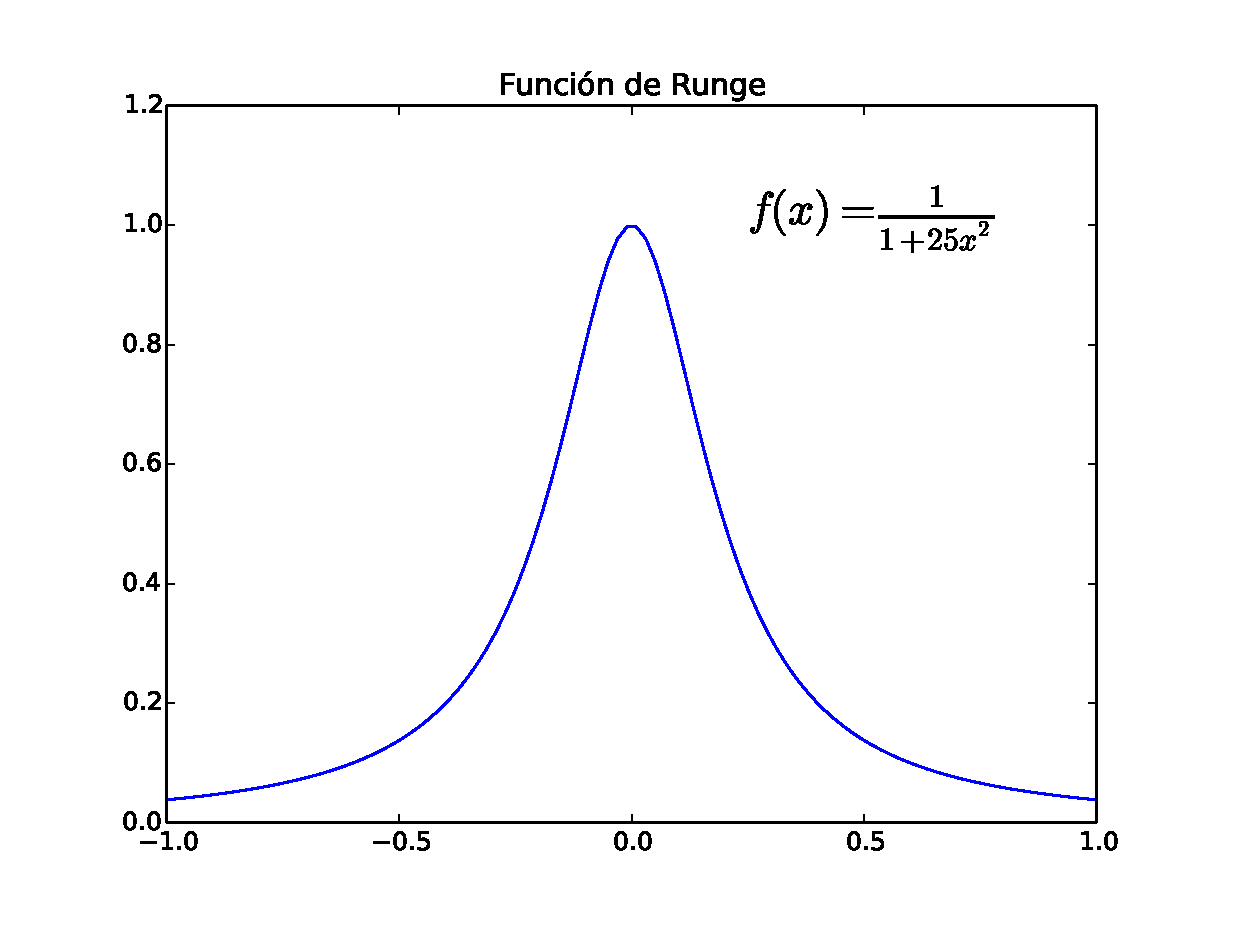
\includegraphics[scale=0.5]{Funcion_Runge_01.eps} 
\end{figure}
\end{frame}
\begin{frame}
\frametitle{Elección de puntos para interpolar}
\begin{figure}
	\centering
	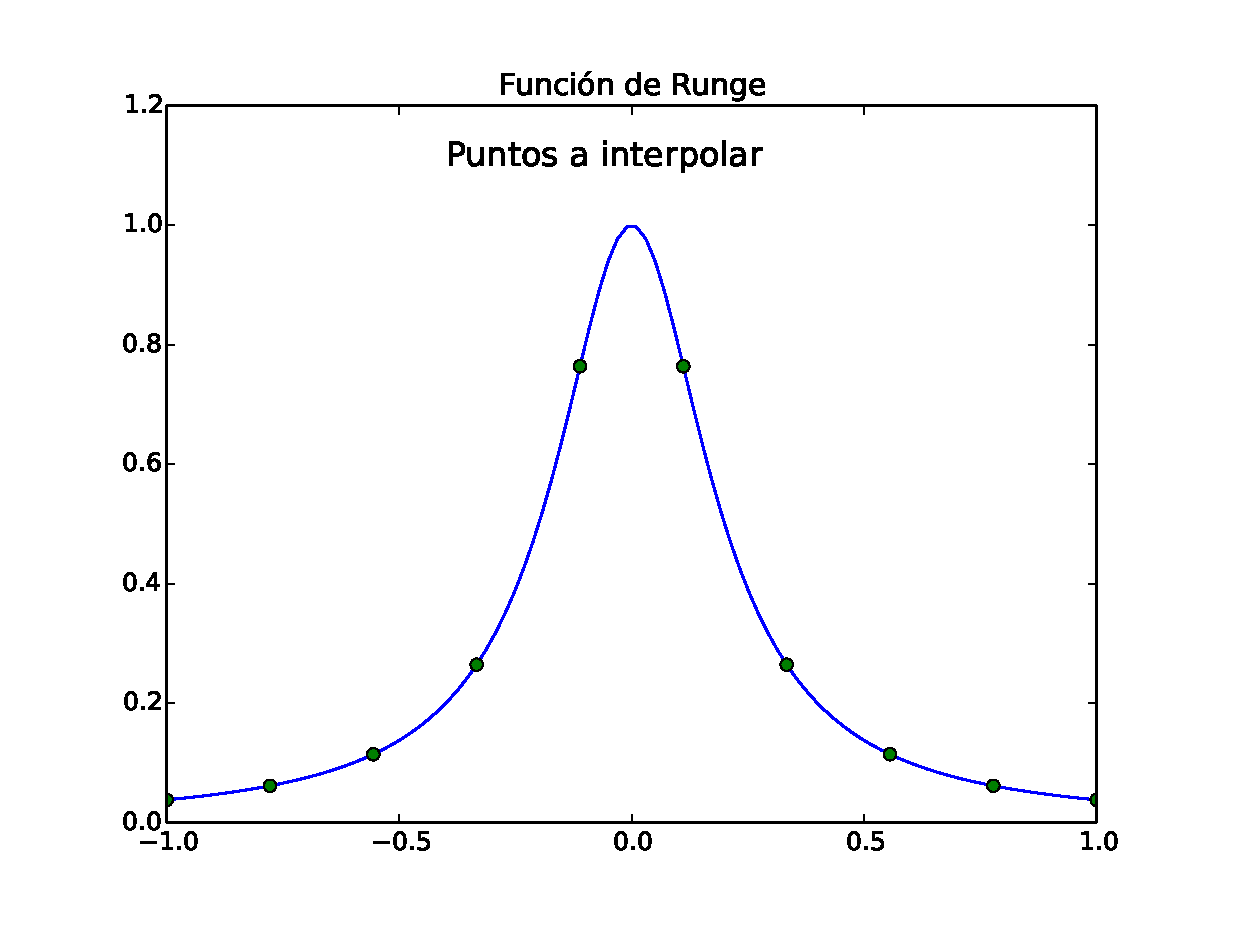
\includegraphics[scale=0.5]{Funcion_Runge_02.eps} 
\end{figure}
\end{frame}
\begin{frame}
\frametitle{Interpolación con Lagrange}
Interpolando los puntos con Lagrange.
\begin{figure}
	\centering
	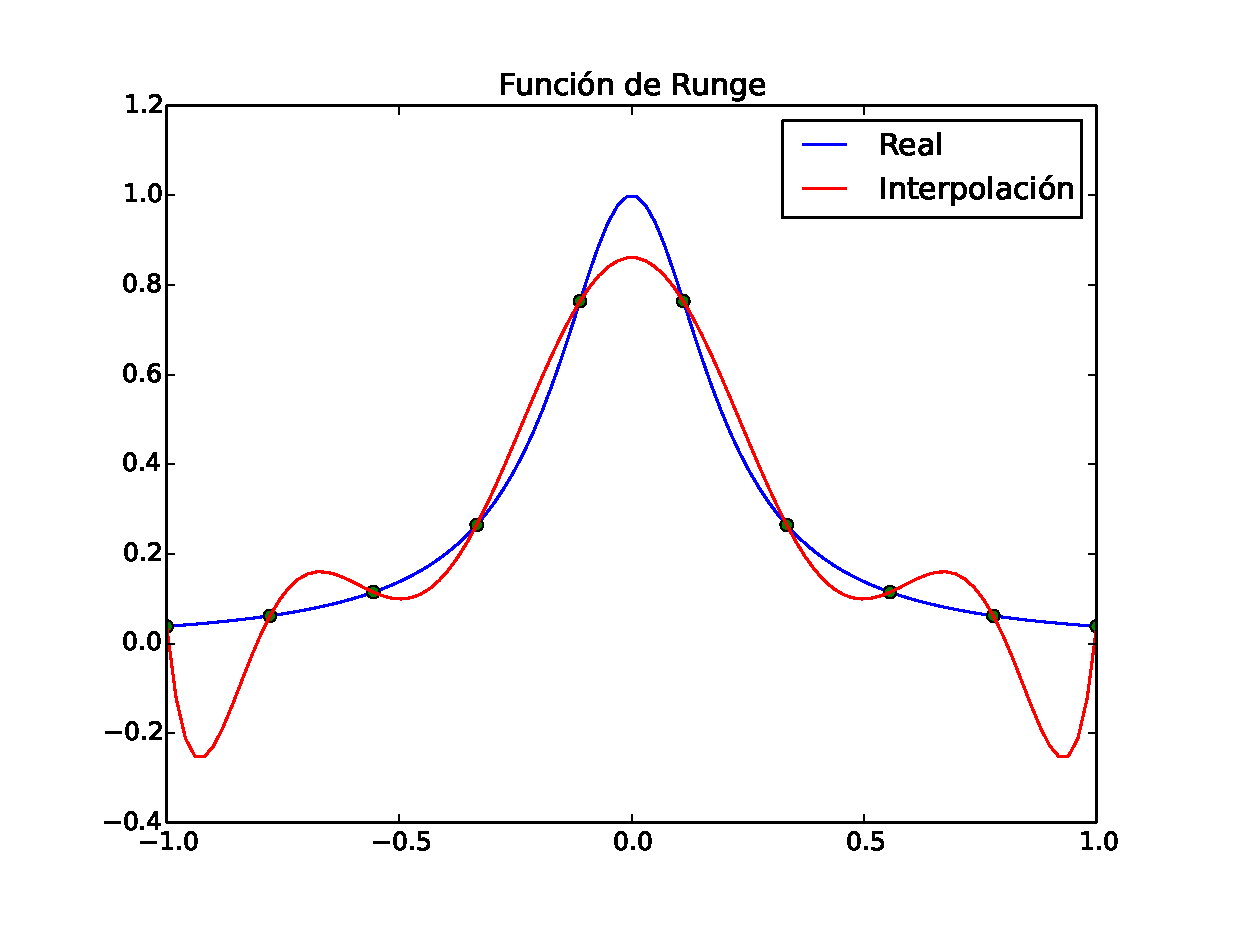
\includegraphics[scale=0.5]{Funcion_Runge_03.eps} 
\end{figure}
\end{frame}
\begin{frame}
\frametitle{¿Qué hacemos al respecto?}
Como hemos visto en la gráfica anterior, la función que resulta del proceso de interpolación ''oscila'' a través de los puntos que deseamos interpolar; aquí el caso es que si aumentamos el grado del polinomio, los resultados serán aún más indeseables.
\\
\medskip
La pregunta obligada es: ¿qué podemos hacer para mejorar la interpolación?
\end{frame}
\section{Uso de splines}
\begin{frame}
\frametitle{¿Qué es un spline?}
En términos nada riguroso, se puede decir que un spline es una función definida por una familia de polinomios ''sociables'', donde el término sociable se usa para indicar que los polinomios que constituyen una función spline, están estrechamente vinculados.
\\
\medskip
El nombre de \emph{spline}, viene del inglés ya que es un instrumento que utilizaban los ingenieros navales para dibujar curvas suaves, forzadas a pasar por un conjunto de puntos prefijados.
\end{frame}
\begin{frame}
\frametitle{Las tres B's de los splines}
El uso de las funciones splines tiene mucha aceptación y popularidad se deben a tres razones básicas:
\begin{enumerate}[<+->]
\item \textbf{Buenos:} Se  pueden usar en la solución de una gran variedad de problemas.
\item \textbf{Baratos:} Ya que su cálculo es muy sencillo y económico.
\item \textbf{Bonitos:} La teoría matemática en que se basan es muy simple y a la vez elegante.
\end{enumerate}
\end{frame}
\begin{frame}
\frametitle{Manejando splines con \python}
Usaremos la librería \texttt{scipy} que contiene varias funciones con las que ahorramos tiempo para manejar splines y ajustar funciones sociables a un conjunto de datos.
\\
\medskip
No está de más que revises la teoría al respecto, en la mayoría de los libros de análisis numérico, podrás encontrar la construcción matemática y formal de los splines.
\end{frame}
\begin{frame}
\frametitle{Funciones para los splines}
Necesitaremos de dos pasos para el uso de splines con \python, de la libería: \texttt{scipy.interpolate}, las cuales son:
\begin{enumerate}
\item \textbf{splrep}: Calcula el spline básico (B-spline) para una curva 1-D.
\\
\medskip
Dados un conjunto de puntos $(x[i],y[i])$ determina una aproximación con un spline suave de grado $k$ en el intervalo $xb \leq x \leq xe$.
\item \textbf{splev}: Evalúa un B-spline o sus derivadas. Dados los nodos y coeficientes de un B-spline, calcula el valor del polinomio suave y sus derivadas.
\end{enumerate}
\end{frame}
\begin{frame}[fragile]
\frametitle{Código}
\begin{lstlisting}
import matplotlib.pyplot as plt
import scipy.interpolate as si
from numpy import *

x = linspace(-1,1,100)
y = 1./(1 + 25*x**2)

def trazador_cub(n):
    xi = linspace(-1,1,n)
    yi = 1./(1 + 25*xi**2)
    tck = si.splrep(xi,yi,s=0)
    return tck
\end{lstlisting}
\end{frame}
\begin{frame}[fragile]
\frametitle{Código}
\begin{lstlisting}
tck = trazador_cub(8)
ys8 = si.splev(x, tck)

tck = trazador_cub(12)
ys12 = si.splev(x, tck)

plt.plot(x,y)
plt.plot(x,ys8,'+g-', label='n=8')
plt.plot(x,ys12,'+r-',label ='n=12')
plt.legend(loc='best')
plt.title('Interpolacion con splines cubicos')
plt.ylim(-0.2,1.2)
plt.show()
\end{lstlisting}
\end{frame}
\begin{frame}
\frametitle{Resultados gráficos}
\begin{figure}
	\centering
	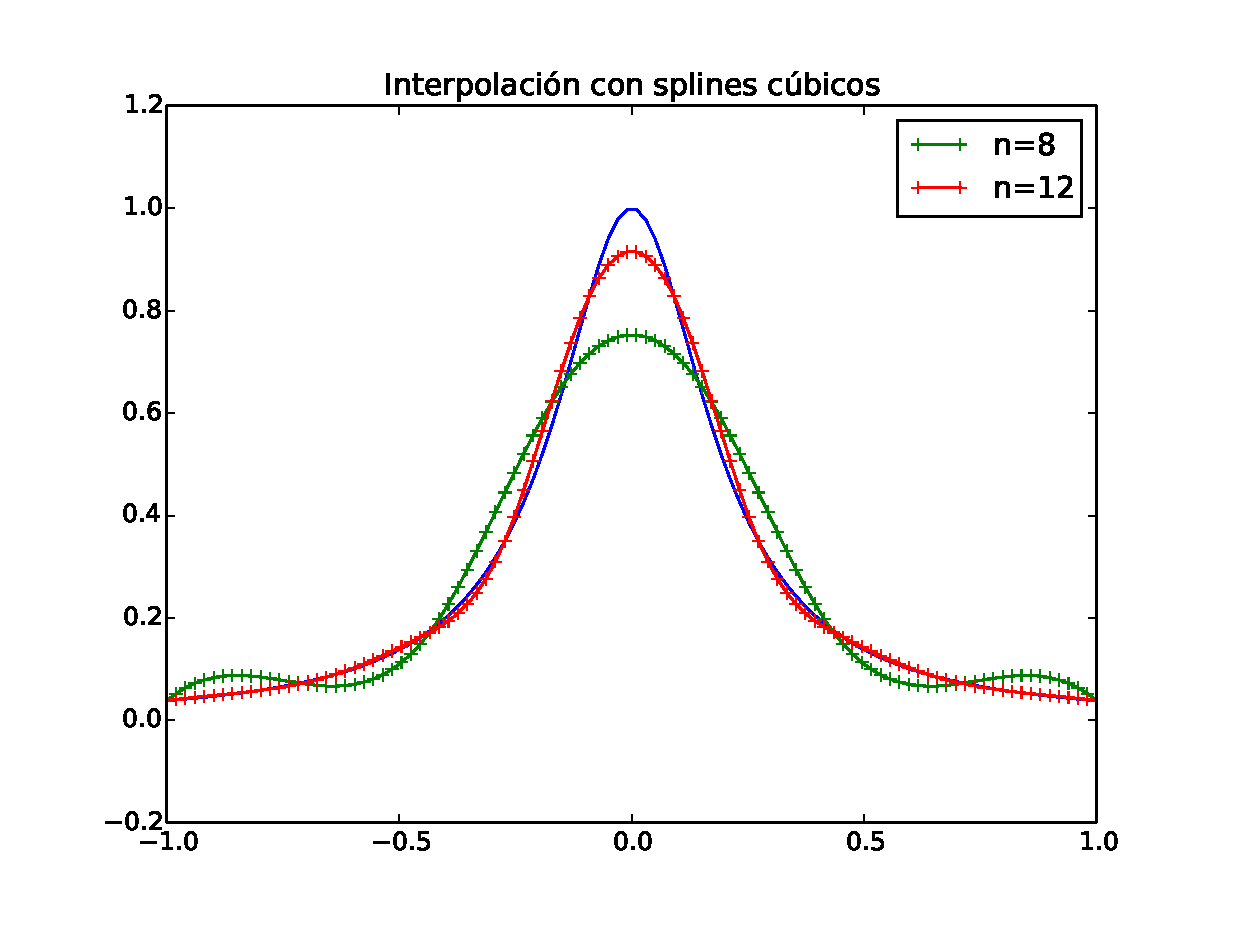
\includegraphics[scale=0.5]{Funcion_Runge_04.eps} 
\end{figure}
\end{frame}
\end{document}
